\chapter{The LHC-ATLAS Experiment}
\section{Large Hadron Collider}
\begin{figure}[tbp]
\begin{center}
%\subfigure[]{
 
\includegraphics[width=1.0\textwidth,keepaspectratio]{figures/detector/CERN}
%}
\caption{
The whole picture of the CERN accelerator complex
}
\label{fig:CERN}
\end{center}
\end{figure}

\section{ATLAS Detector}
The ATLAS Detector [11] was designed to measure all standard model particles 2) produced by LHC collisions, a schematic overview of the whole ATLAS detector is shown in Figure 3.2. The detector position surrounding the beam pipe called barrel, and those aligned at the high η regions are referred to as end-caps.
The magnet system and the luminosity detector are introduced in Section 3.3.1 and 3.3.2, respectively. Four major subsystems, the inter tracker, the calorimeters, the muon spectrometer, and the trigger & data acquisition system are described.
\begin{figure}[tbp]
\begin{center}
%\subfigure[]{
 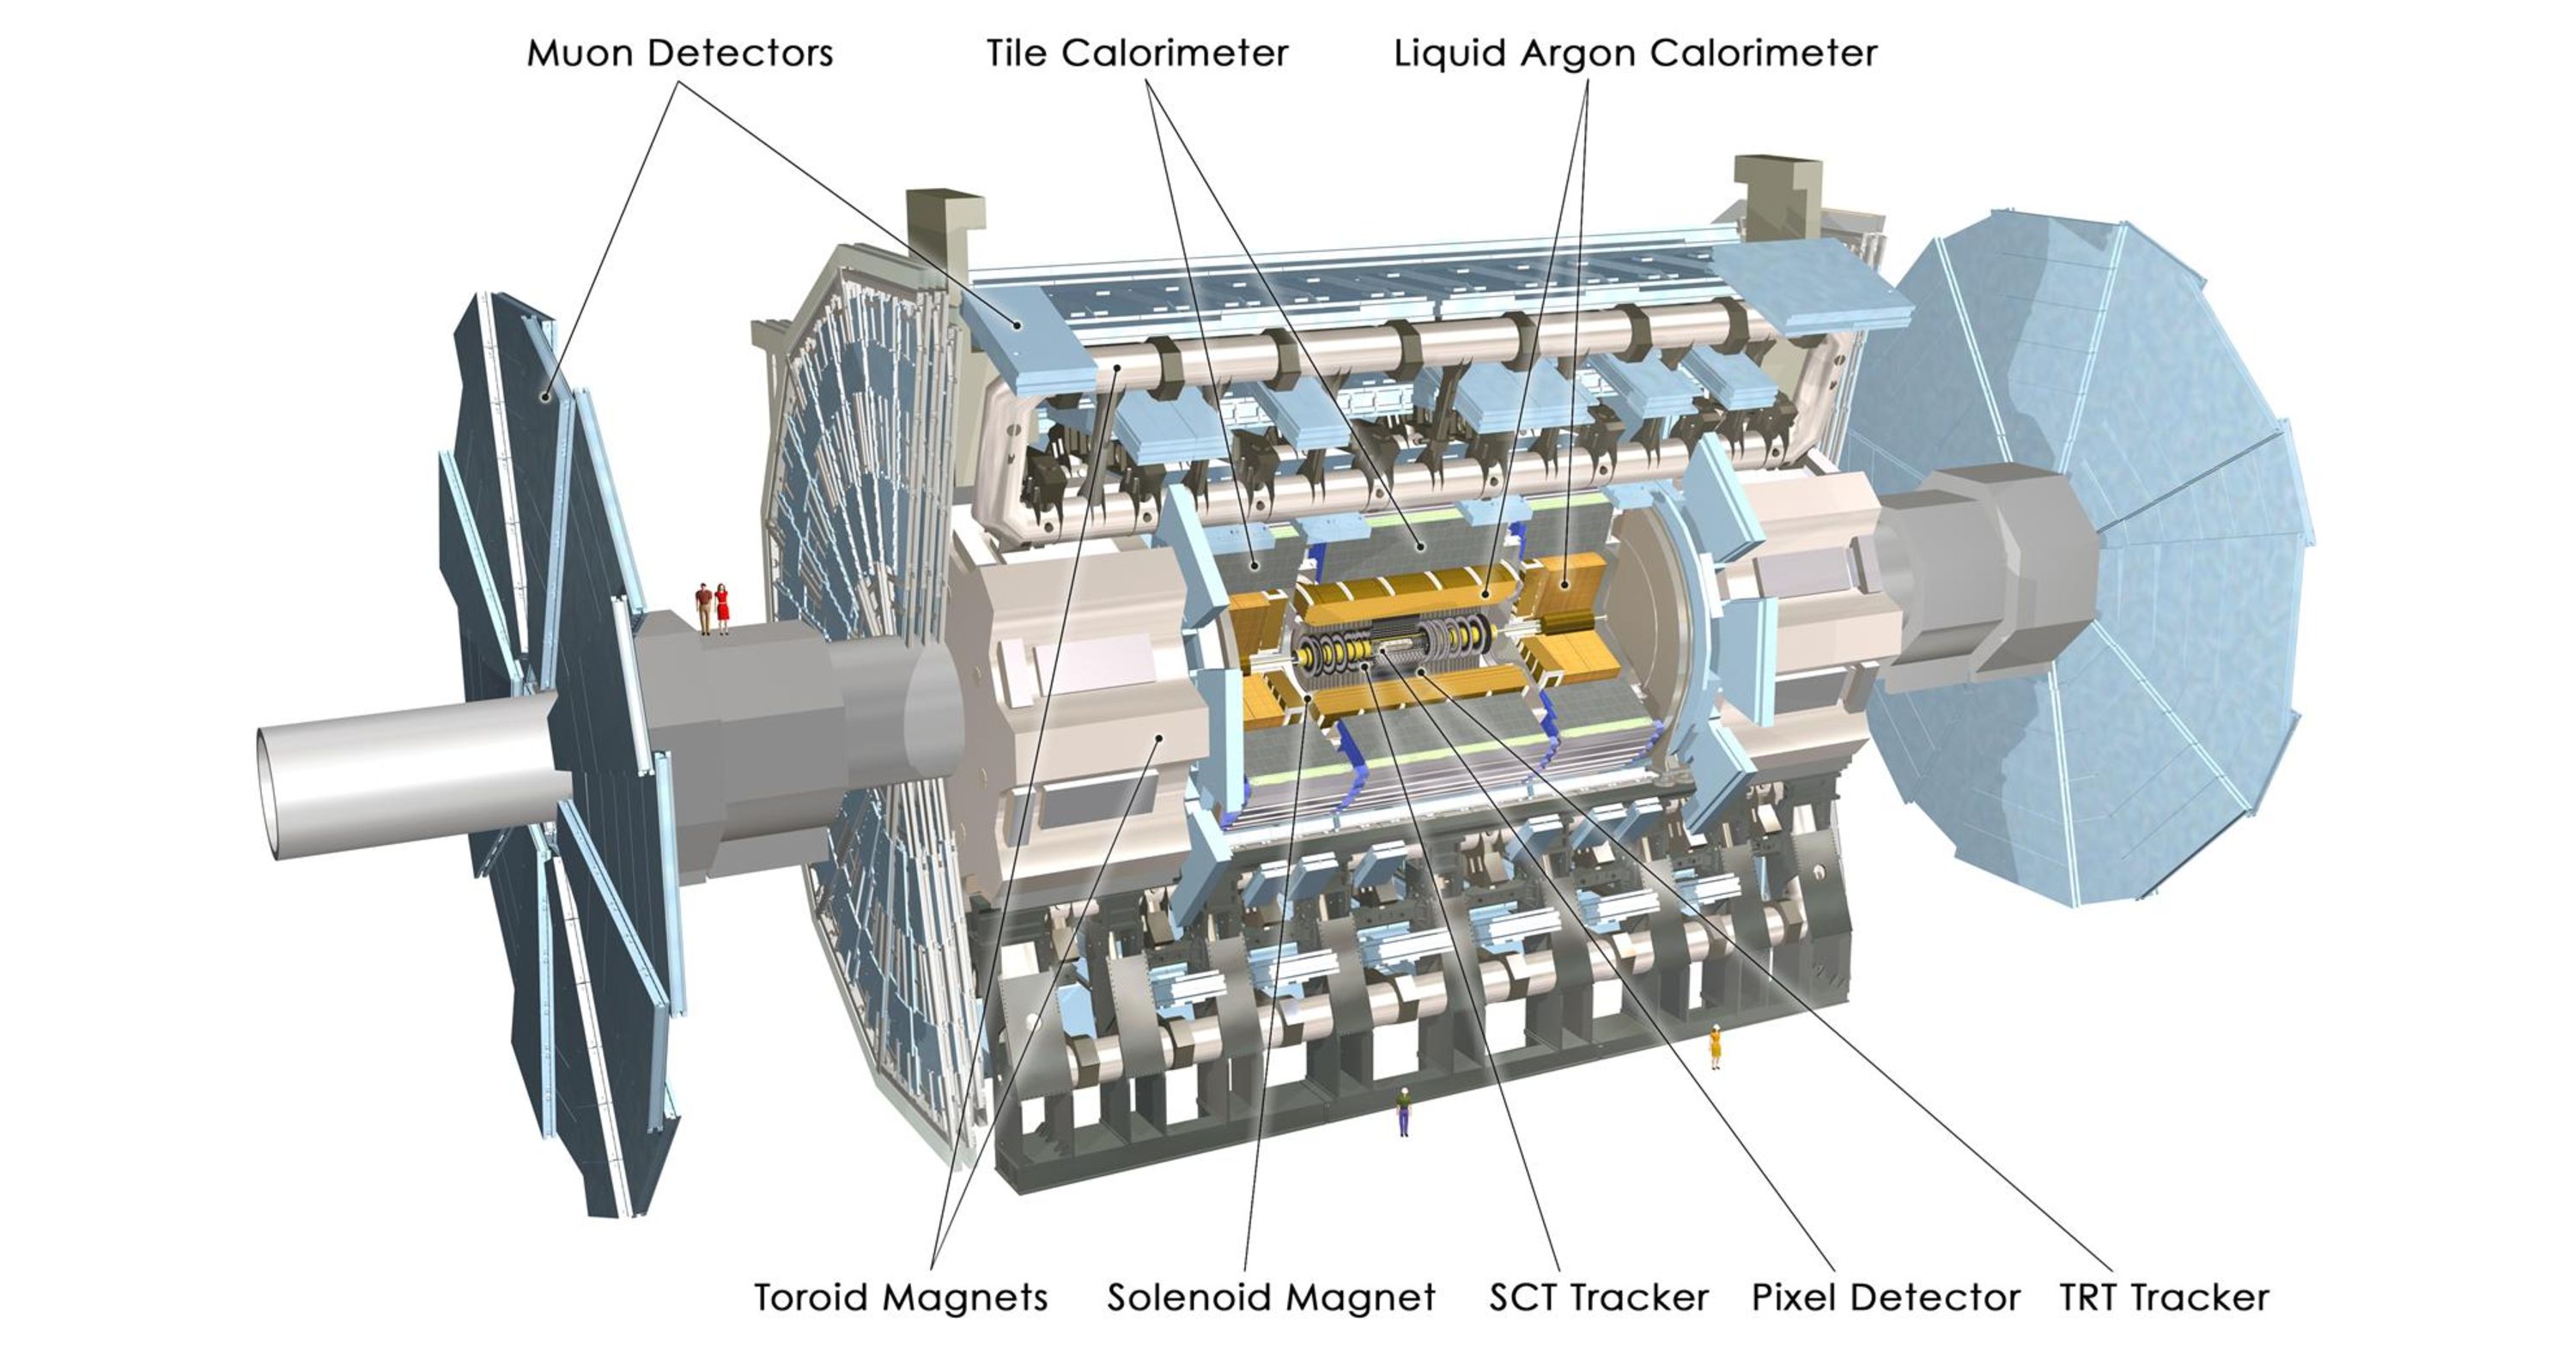
\includegraphics[width=1.0\textwidth,keepaspectratio]{figures/detector/ATLAS}
%}
\caption{
The whole picture of the ATLAS detector
}
\label{fig:CERN}
\end{center}
\end{figure}

\subsection{Magnet}
The ATLAS magnet system consists of four large superconducting magnets with a dimension of 22 m in diameter and 26 m in length with a stored energy of 1.6 GJ. A solenoid aligned on the beam axis generates 2 T axial magnetic field for the inner detector, which placed inside the calorimeter system. A toroid on the barrel and two toroids on the end-caps are installed and those provide 0.5 and 1T magnetic fields for muon detectors, respectively.
\subsection{Inner Tracker}
The tracking, the reconstruction of charged particle trajectory, is performed by the inner detectors. Those consist of three subsystems, Pixels, SCT, and TRT. The schematic graphs of the inner detectors are illustrated in Figure. Each subsystem is introduced as follows.
\subsubsection{Pixel Detector}
The most inner tracker system, the Pixel Detectors is made of four cylindrical layers of silicon pixel modules covering inner radii of 33.25-122.5 mm and |η| < 2.5. The most inner pixel layer called IBL(Insertable B-Layer) is newly added before the 2015 run for the better tracking quality and radiation endurance. The IBL is installed at 33.25 mm from the beamline, and it has 50 × 250 μm pitch pixels and is qualified for a radiation hardness up to 5 × 1015 1-MeVneqcm−2 4) corresponding to 550 fb−1 with a peak luminosity of 3 × 1034 cm−2s−1 [67]. The next three outer cylindrical layers and
two end-caps each with three discs cover |η| <∼ 2.5 by 1744 pixel sensors with 250 μm thick and size 2 of 50 × 400 μm . Each sensor has 47232 readout channels. The sensors are operated in the temperature between −5 and −10 ◦C to reduce leakage current.
\subsubsection{SCT Detector}
The subsystem placed at the next outer of the Pixel Detector is called SCT (Semiconductor Tracker) made by silicon microstrips located at 30-50 cm from the beamline. 80 μm pitch microstrips printed on the front and back with ±20 mrad angled each other to reconstruct the two-dimensional loca- tion of the energy deposit. Modules are installed as four layers, there are 2112 modules on the barrel and 1976 modules in the end-cap regions.
\subsubsection{TRT Detector}
The TRT made by transition radiation detectors located 50-100 cm from the beamline covering |η| < 2.0. Drift tubes with a dimension of 4 mm diameter and 144 cm length are filled by a mixture of Xenon (70\%), CO2 (27\%), and Oxygen (3\%). The TRT used not only tracking but also the separation between electrons and pions by using the difference of intensity of transition radiation characterized by those Lorentz factors.
Hits on the above detectors are collectively used for the tracking. Designed tracking resolution is σpT /pT = 0.05\%pT ⊕ 1\% with coverage of |η| ± 2.5.
\subsection{Calorimeters}
The calorimeters measure the energy of particles. Two major components, Electromagnetic Calorimeter and Hadron Calorimeter are built outside of the inner tracker as illustrated in Figure.
\subsubsection{ElectroMagnetic Calorimeter}
The electromagnetic calorimeter is made by lead and liquid Argon for
design consideration. The total thickness of the EM calorimeter is > 22 radiation lengths (X0)
detecting electromagnetic showers. It is subdivided into the barrel (|η| < 1.4) and end-caps (1.4 <
in the barrel and > 24 X0 in the end-caps. The approximate 9.7 interaction lengths (l ) of active
|η| < 3.2) by pseudorapidity. The electromagnetic calorimeter is shaped like an accordion to cover
calorimeter in the barrel (10 l in the end-caps) are adequate to provide good resolution for high-
complete φ ranges without any cracks and to extract signals rapidly at the tail or head of the electrodes.
energy jets (see table 1.1). The total thickness, including 1.3 l from the outer support, is 11 l
Both the barrel and end-cap electromagnetic calorimeters are divided into three longitudinal layers. The
at h = 0 and has been shown both by measurements and simulations to be sufficient to reduce granularity and radiation length(X ) for those at η = 0 are represented as ∆η × ∆φ = 0.003 × 0.1
punch-through well below the irreducible level of prompt or decay muons. Together with the large andX =4.3,∆η×∆φ=0.025×0.025andX =m1i6ss,and∆η×∆φ=0.05×0.025andX =2.0
h-coverage, this thickness will also ensure a good E measurement, which is important for many
A schematic diagram for the barrel calorimeter cells is shown in Figure 3.6. The energy deposits in physics signatures and in particular for SUSY particle searches. the liquid Argon gap induce electric current proportional to the deposited energy. The triangular input current pulse which has a length of the maximum drift time (typically 450 ns) is shaped by a bipolar filterLAr electromagnetic calorimeter
in front-end boards [68] to avoid overlap with the next collision as shown in Figure 3.7. In order to cover The EM calorimeter is divided into a barrel part (|h| < 1.475) and two end-cap components the required dynamic range, three different gains, high, medium and low are implemented corresponding (1.375 < |h| < 3.2), each housed in their own cryostat. The position of the central solenoid in to 100, 10, and 1 linear gain scales, respectively. The amplified signals are sampled at 40 MHz and front of the EM calorimeter demands optimisation of the material in order to achieve the digitized by a 12-bit analog-to-digital (ADC) converter.
\subsubsection{Hadron Calorimeter}
The hadronic calorimeter is placed outside of the electroweak calorimeter to detect the hadronic shower made by hadrons. It is separated into the barrel (|η| < 1.7), end-caps (1.5 < |η| < 3.2), and forward (3.1 < |η| < 4.9). The barrel is made by steal absorbers, scintillating tiles, and photomultipliers, which divided into three longitudinal layers having approximately 1.5, 4.1, and 1.8 interaction length thicks at η = 0. Each readout cell is segmented by ∆η × ∆φ = 0.1 × 0.1 in the first and second layers and 0.1 × 0.2 in the third layer. A schematic diagram is shown in Figure 3.6. The end-cap calorimeters are a sampling calorimeter made by liquid Argon and copper plates. Cryostats are shared with the end-cap electromagnetic calorimeters and the forward hadron calorimeters. The size of areadoutcellis∆η×∆φ = 0.1×0.1inthe1.5 < |η| < 2.5and0.2×0.2inthe2.5 < |η| < 3.2. The forward hadron calorimeter the sampling calorimeter is made by liquid Argon and metal plates and is separated into three layers. The first layer uses copper plates as absorbers the same as the end-cap calorimeter. The second and third layer employs tungsten as absorbers. The absorption lengths are 2.66, 3.68 and 3.60 for each layer.
The hits in the calorimeters are collectively used in analyses to reconstruct the energy of particles. The designed energy resolution for the electromagnetic calorimeter is σE/E = 10\%/√E ⊕ 0.7\% with cov- erage of |η| < 3.2, and the barrel and end-cap hadron calorimeter are designed to be a resolution of σE/E = 50\%/√E⊕3\% with coverage of |η| < 3.2. Design resolution of the forward hadron calorimeter is σE/E = 100\%/√E ⊕ 10% covered 3.1 < |η| < 4.9.
\subsection{Muon Spectrometer}
The muon spectrometers are placed on the most outside of the ATLAS detector to detect punch-through minimum ionization particles. It is used for both identification and triggering. Four types of modules are constructed as shown in Figure 3.8. The major parameters of them are shown in Table.
\subsection{Trigger and Data Aquisition System}
It is impossible to store all information provided detectors for every 25 ns collision, the trigger system is installed to select physically motivated events as shown in Figure 3.9. Details of the trigger system are summarized in References [69, 70]. The ATLAS trigger system consists of a hardware-based Level-1 trigger (L1) and software-based High-Level Trigger (HLT).
The L1 consists of L1Calo, L1Muon, L1Topo, and CTP (central trigger processor) for triggering elec- miss 5)
trons, muons, hadronic taus, photons, jets, and ET . The L1Calo exploits 7168 calorimeter towers which made by the harsh granularity of ∆φ × ∆η = 0.1 × 0.1 for fast readouts. For the L1 electron and L1 photon, 2 × 2 core towers and 12 surrounded towers of electromagnetic calorimeters are used for cap- turing the electron energy and calculating isolation requirement, respectively. For the L1 jet, wider 4 × 4 core towers of electromagnetic and hadron calorimeters are collectively used since the jet is typically wider than the showers for electrons and photons. The L1Muon makes use of RPC and TGC hits and fires if there is a coincidence between different chambers based on the predefined look-up-tables. Such
reconstructed L1 objects by the L1Calo and L1Muon are sent to the L1Topo. The L1Topo performs se- lections based on kinematical information about L1 objects. Then all information calculated by L1Calo, L1Muon, and L1Topo are sent to the CTP to make trigger decisions about up to 512 trigger items and defines the region of interests (ROI). The latency for the whole L1 trigger system is 2.5 μs.
The HLT reconstructs objects with offline like algorithms6) with the full detector information around ROI in a large CPU farm (40,000 processor cores) and providing about 2500 independent trigger chains. Some triggers are worked as a prescale trigger. A prescale trigger is the one which fired at random 1/n events satisfying the trigger selection, where n referred to as prescale factor. The processing time of the HLT is typically within 300 ms.
L1 and HLT trigger rate decompositions for a typical fill are shown in Figure 3.10. In the L1, half of the
total trigger rate is occupied by the lepton triggers. The Emiss trigger has a dependence on instantaneous T
luminosity, hence the HLT trigger rate was dominant at the beginning of collisions, but it was suppressed at the end of collisions.